\phantomsection
\chapter{Viola-Jones}

\noindent Viola-Jones algorithm is "a visual object detection framework that is capable of processing images extremely rapidly while achieving high detection rates". 3 main points characterize this algorithm. The first one is the use of what is called an "Integral image". It is a new representation of the image and it allows the features used to be computed very quickly. The second one is the use of a learning algorithm based on AdaBoost. It results in giving extremely efficient classifiers. The third and last one is the use of a method to combine classifiers. This method combine classifiers in "cascade". It allows to focus on the promising object-like regions by discarding the background in a very quick way \cite{VIO01}.
\newline

\phantomsection
\section{Overview}

\vspace{\baselineskip}
\noindent The Viola-Jones algorithm works as following \cite{DIN08}:

\begin{itemize}
  \item "The Viola-Jones detector is a strong, binary classifier build of several weak detectors"
  \item "Each weak detector is a simple binary classifier"
  \item During the learning part, a cascade of weak classifiers is used and trained in order to attained the desired hit/miss rate using the learning algorithm based on AdaBoost
  \item The input image is divided in several rectangular sub-regions in order to detect objects. The cascade computes each of these sub-regions
  \item To classify a sub-region as "positive", it has to go through all of the stages of the cascade
  \item All the process involving the sub-regions is repeated at different scales
\end{itemize}

\phantomsection
\section{Haar features}

\vspace{\baselineskip}
\noindent The features used by Viola and Jones are called Haar features and are based on Haar wavelets. Haar wavelets are single wavelength square waves. It is composed of one high interval and one low interval. In two dimensions, a square wave is represented by a pair of adjacent rectangles: one rectangle that is light and one rectangle that is dark. The true Haar wavelets are not the one used for this rectangle combinations that is used for visual object detection. They use instead rectangle combinations that are better suited to recognition tasks. That is because of this difference that these features are called Haar features rather than Haar wavelets (they can also be called Haarlike features) \cite{HEW07}.
\newline

\noindent For example, the figure~\ref{haar_features_first_2_stage} shows the first two Haar features in the original Viola-Jones cascade \cite{HEW07}. These are all features from the original set of features. In figure~\ref{haar_features_extended}, there is an example of features from the extended set of features \cite{DIN08}. In the figure~\ref{haar_features_early_stage} , it is an example of a early stage in the Haar cascade. Each black and white rectangle represents a feature. And that is what the algorithm hunts for in the image \cite{HAR12}.
\newline

\begin{figure}[!h]
\begin{center}
\noindent 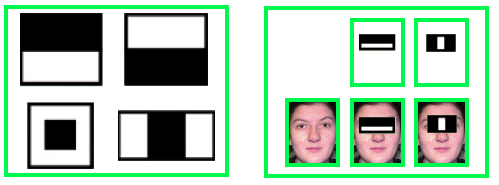
\includegraphics[scale=0.9]{figures/haar_features_first_2_stage} 
\newline
\caption{Example of the first two Haar features}
\label{haar_features_first_2_stage}
\end{center} 
\end{figure}

\begin{figure}[!h]
\begin{center}
\noindent 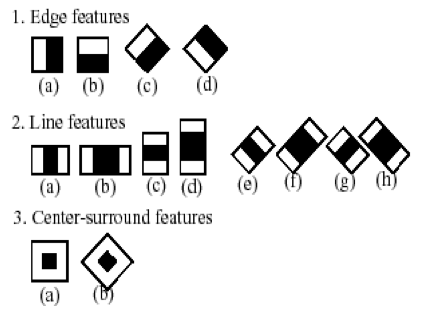
\includegraphics[scale=0.6]{figures/haar_features_extended} 
\newline
\caption{Extended set of features}
\label{haar_features_extended}
\end{center} 
\end{figure}

\begin{figure}[!h]
\begin{center}
\noindent 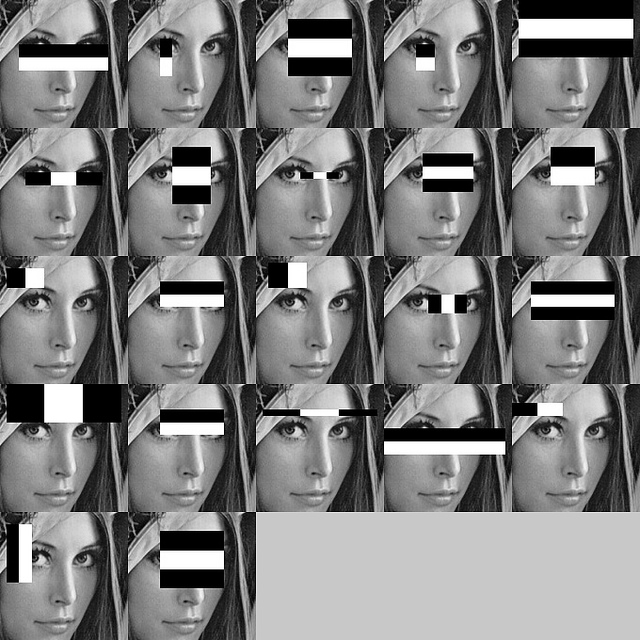
\includegraphics[scale=0.5]{figures/haar_features_early_stage} 
\newline
\caption{Example of an early stage in the Haar cascade}
\label{haar_features_early_stage}
\end{center} 
\end{figure}

\noindent To detect if a Haar feature is present or not, basic subtraction is used. The subtraction consists in subtracting the average pixel value of the dark-region from the average pixel value of the light-region. Then it is a simple comparison. The result of the subtraction is compared with a threshold. If the result is above the threshold, then the feature is considered as present and it can go to the next stage \cite{HEW07}. There is about 20 to 30 different stages to detect the presence of Haar features. The first stage is a very coarse scan of the image. The second stage is more detailed, the third stage is once again more detailed and harder to pass, the fourth stage is even harder and it goes on and on till the end. The more it moves froward into the cascade, the more it becomes harder. The features become increasingly complex and larger. All this processing takes indeed more time to compute \cite{HAR12}.
\newline

\noindent For example, the figure~\ref{haar_feature_later_stage} shows the later stage in the Haar cascade. There are many more patterns of black and white rectangles that need to match the input image \cite{HAR12}.
\newline

\begin{figure}[!h]
\begin{center}
\noindent 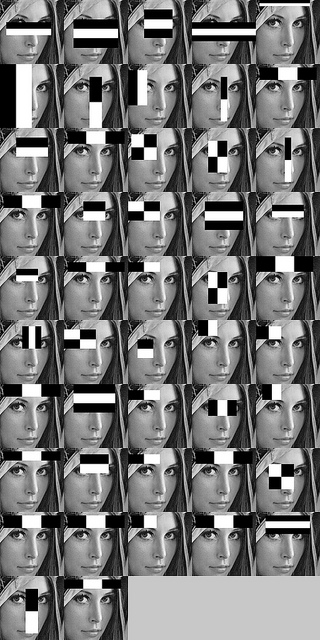
\includegraphics[scale=0.8]{figures/haar_feature_later_stage} 
\newline
\caption{Example of the later stage in the Haar cascade}
\label{haar_feature_later_stage}
\end{center} 
\end{figure}

\noindent It exists three kinds of feature that Viola and Jones use: a two-rectangle feature, a three-rectangle feature and a four-rectangle feature. To find the value of the two-rectangle feature, it consists in the difference between the sum of the pixels that are in the two rectangular regions. The regions (or rectangles) are the same: they have the same size and the same shape. And they are horizontally or vertically adjacent. The three-rectangle feature are calculated by the sum of the pixels of the two outside rectangles subtracted from the sum of the pixels in the center rectangle. The last kind of feature is the four-rectangle feature consists in the difference between the diagonal pairs of rectangles \cite{VIO01}.
\newline

\noindent For example, the figure~\ref{haar_feature_description} shows the different kinds of rectangle features used by the Viola-Jones algorithm. The images (A) and (B) show the two-rectangle features. The image (C) shows the three-rectangle feature, and the image (D) shows the four-rectangle feature \cite{VIO01}.
\newline

\begin{figure}[!h]
\begin{center}
\noindent 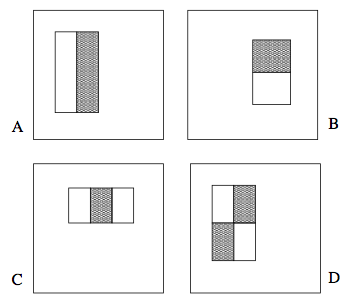
\includegraphics[scale=0.6]{figures/haar_feature_description} 
\newline
\caption{Example of the different kinds of rectangle features}
\label{haar_feature_description}
\end{center} 
\end{figure}

\noindent Viola and Jones admit that rectangle features can be considered as primitive features. In contrast with other features, rectangle features are quite coarse (even though they are sensitive to the presence of edges, bars and other simple image structure). It appears that however, a rich image representation is provided by this set of rectangle features and furthermore this representation supports effective learning. In comparison with the extreme computational efficiency provided by rectangle features, their limited flexibility is not much of a problem \cite{VIO01}.
\newline

\phantomsection
\section{Integral image}

\vspace{\baselineskip}
\noindent Viola and Jones used an intermediate representation of an image that they called "integral image". This integral image allows to compute very quickly the rectangle features \cite{VIO01}. This technique allows to determine the presence or absence of hundreds of Haar features. It can be determined for every image location and for several scales efficiently. In general, adding small units together is what is called "integrating"; here, the small units are pixel values. The sum of all the pixels above and to the left of each pixel is the the integral value. And this value can be found for each pixel. That is why this technique is efficient: the entire image can be integrated only with a few calculations per pixel. This integration starts at the top left corner and go through all the image to the right and down \cite{HEW07}.
\newline

\noindent It means that the integral image, at location $ x,y $ contains the sum of the pixels above and on the left of $ x,y $, $ x,y$ included: \[ ii(x,y) = \sum_{x' \leq x,y' \leq y} i(x',y') \] where $ ii(x,y) $ is the integral image and $ i(x,y) $ is the regional image. In the figure~\ref{integral_image_description}, the value of the integral image at point $ (x,y) $ is the sum of all the pixels above and on the left \cite{VIO01}. 
\newline
	
\begin{figure}[!h]
\begin{center}
\noindent 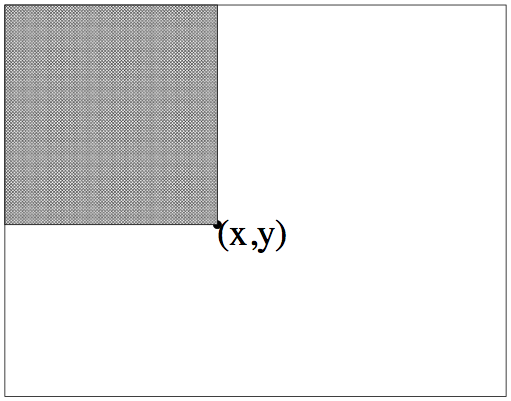
\includegraphics[scale=0.5]{figures/integral_image_description} 
\newline
\caption{Integral image}
\label{integral_image_description}
\end{center} 
\end{figure}
	
\noindent Using the following pair of recurrences: 
\begin{equation}
s(x,y) = s(x,y - 1) + i(x,y)
\end{equation}
\begin{equation}
ii(x,y) = ii(x - 1,y) + s(x,y)
\end{equation}
(where $ s(x,y) $ is the cumulative row sum, $ s(x,-1) = 0 $, and $ ii(-1,y) = 0 $) the integral image can be computed in one pass over the original image. 
\newline

\noindent Thanks to the integral image, any rectangular sum can be calculated in four array references. In the figure~\ref{integral_image_four_array}, the sum of the pixels in rectangle D can be calculated with four array references. The value of the integral image at the point 1 is the sum of the pixels in rectangle $ A $. The value at the point 2 is $ A + B $, at the point 3 is $ A + C $, and at the point 4 is $ A + B + C + D $. The sum in D can then be computed as $ 4 + 1 - (2 + 3) $ \cite{VIO01}. 
\newline

\begin{figure}[!h]
\begin{center}
\noindent 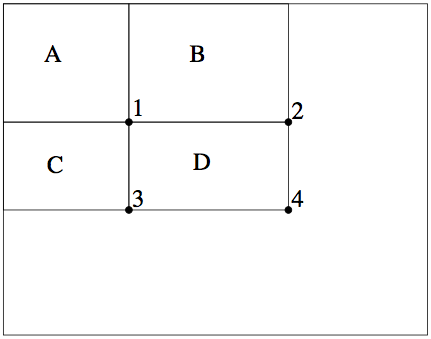
\includegraphics[scale=0.6]{figures/integral_image_four_array} 
\newline
\caption{Integral image with four array references}
\label{integral_image_four_array}
\end{center} 
\end{figure}

\phantomsection
\section{Weak classifiers and AdaBoost}

\vspace{\baselineskip}
\noindent Features are extracted from a sub-region of an input image. This sub-region has a size that is usually of 24 by 24 pixels. Each of all the features types are moved and scaled across the entire input image (In a 24 pixel by 24 pixel sub-region, it means that there are about 160,000 possible combinations to process) \cite{SMY07}.
\newline

\noindent AdaBoost is a machine-learning method used by Viola and Jones in order to select the specific Haar features to use. It is also used to set the threshold levels. This method is based on the combination of many weak classifiers to form a strong one. It is called a weak classifier because this kind of classifiers obtains the right answer only a little more often than a random guess would which is not particularly good. The purpose of using so many weak classifiers is to get a right answer with a higher rate of success. All of this is based on the verified hypothesis that if each of the weak classifiers pushes the final answer a little bit in the right direction each time, it means that at the end, the correct answer is obtained. This combination of several weak classifiers represents a strong one \cite{HEW07}. 
\newline

\noindent AdaBoost works the following way: it chooses a set of weak classifiers that are going to be combined and assigns  to each of these classifiers a weight (see figure~\ref{haar_feature_adaboost}). The result of this weighted combination is a strong classifier \cite{HEW07}. One of the difficulties and challenges for this learning algorithm is to associate a large weight for each good classifier and a smaller weight for each poor classifier. In order to succeed in selecting a small group of good classifiers but with still significant variety, AdaBoos is quite an aggressive algorithm \cite{VIO01}.
\newline

\begin{figure}[!h]
\begin{center}
\noindent 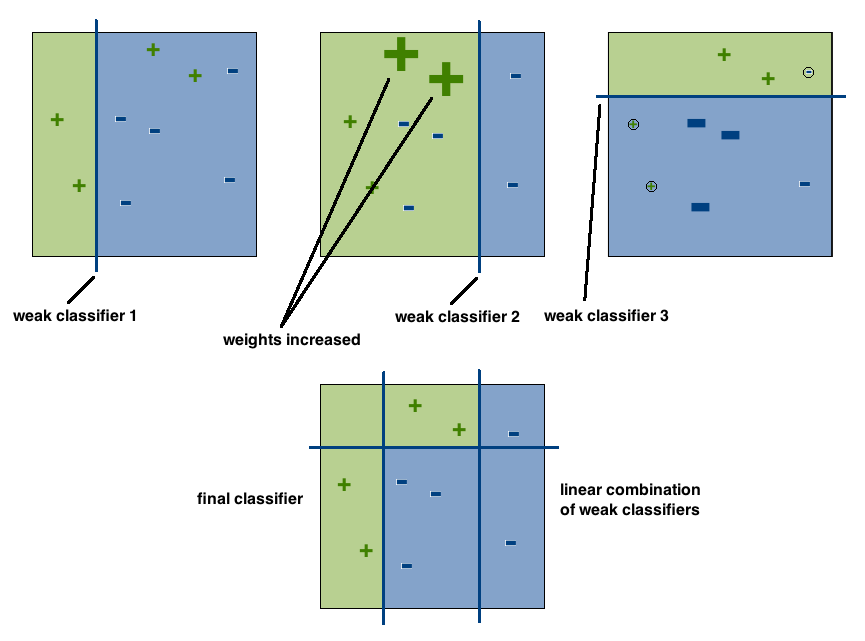
\includegraphics[scale=0.6]{figures/haar_feature_adaboost} 
\newline
\caption{AdaBoost method}
\label{haar_feature_adaboost}
\end{center} 
\end{figure}

\noindent Experiments have been tested with a classifier constructed from 200 features and using AdaBoost. The result would give reasonable results. The detection rate of the classifier was of 95\% and it obtain only 1 false positive in 14084 on a testing dataset (see figure~\ref{haar_feature_example_result})\cite{VIO01}.
\newline

\begin{figure}[!h]
\begin{center}
\noindent 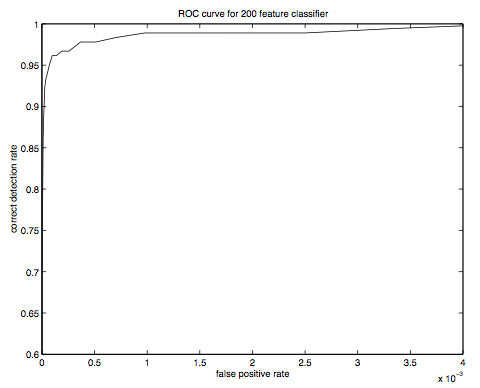
\includegraphics[scale=0.8]{figures/haar_feature_example_result} 
\newline
\caption{Receiver operating characteristic (ROC) curve for the 200 feature classifier}
\label{haar_feature_example_result}
\end{center} 
\end{figure}

\noindent With this experiment, it is an initial evidence that the 200-feature classifier is an efficient technique for object detection. It means that a boosted classifier constructed from rectangle features is also an efficient technique for object detection. The results of this experience are convincing in terms of detection. But they may not be sufficient for real-world tasks. This boosted classifier requires 0.7 seconds to scan an $ 384\times288 $ pixel image. So regarding the computation time, it is probably faster than any other system already published. In order to improve the system so that it will suit to real-world tasks, the detection performance must be improved. But the most straightforward method to do that is to add features to the classifier and doing that will immediately decrease the speed of this system; it will increase computation time \cite{VIO01}.
\newline

\phantomsection
\section{Classifiers cascade}

\vspace{\baselineskip}
\noindent What Viola and Jones did to classify image regions and sub-regions in an efficient way is to combine AdaBoost classifiers as a filter chain. It is constructed as a cascade and that is why Viola and Jones named it  "Classifiers cascade" comes from. This chain is composed for each filter of a separate AdaBoost classifier that has a fairly small number of weak classifiers. As in figure~\ref{haar_feature_cascade}, the classifier cascade represents a chain of filters. If an image sub-regions makes it through the whole cascade, it is classified as "Face". If not it is classified as "Not Face" \cite{HEW07}. Using this algorithm with the classifiers cascade method allows to reduce significantly the computation time and to increase significantly the detection performance \cite{VIO01}.
\newline

\begin{figure}[!h]
\begin{center}
\noindent 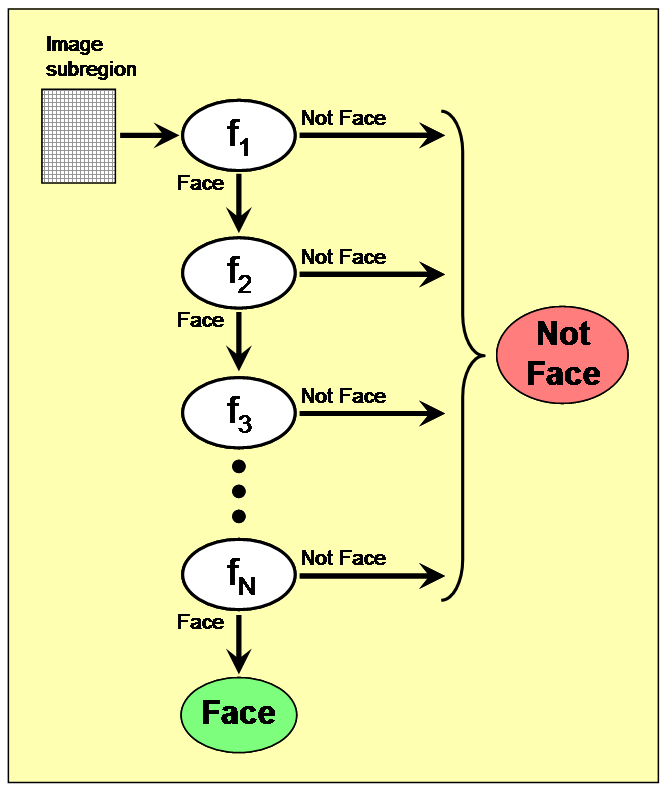
\includegraphics[scale=0.5]{figures/haar_feature_cascade} 
\newline
\caption{Cascade of boosted classifiers}
\label{haar_feature_cascade}
\end{center} 
\end{figure}

\noindent Tests were made to see if the cascade method was feasible. To do that, two simple detectors were trained. One of them was a 200-feature classifier and the other one was a cascade of 10 20-feature classifiers. Figure~\ref{haar_feature_cascade_example_result} gives the ROC curves that compare the performance of the two classifiers. Between the two classifiers, regarding their accuracy, the difference is little and not significant. On the other hand, regarding their speed, the difference is large and significant. The classifier cascade is about 10 times faster. This is because as soon as the first stage, most of the non-faces are discarding so in all the next stage, the classifier never evaluate them again \cite{VIO01}.
\newline

\begin{figure}[!h]
\begin{center}
\noindent 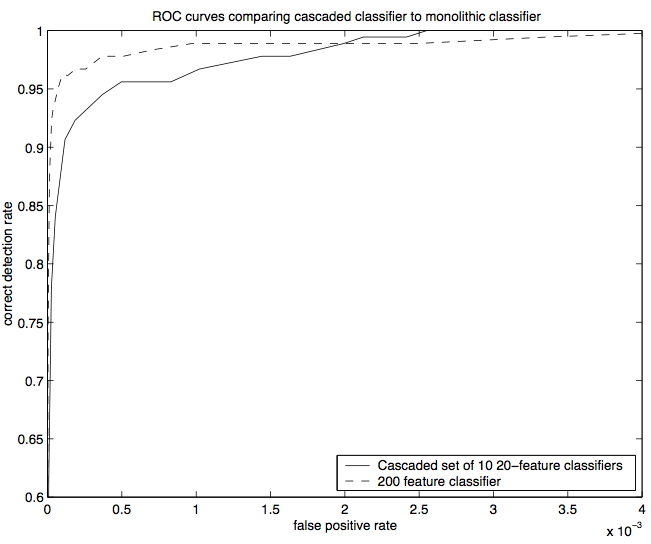
\includegraphics[scale=0.6]{figures/haar_feature_cascade_example_result} 
\newline
\caption{ROC curves of a 200-feature classifier and of a classifier cascade that contains 10 20-feature classifiers}
\label{haar_feature_cascade_example_result}
\end{center} 
\end{figure}

\noindent The cascade method has been made in a way that there must not be false negative. That means that a face must not be classified as "Not Face". To do that, the assistance threshold has been set low for each level. This way, in the training set, it is low enough to pass all or almost all face examples. All the training images that passed previous stages are classified by filters trained to do it for each level. A region is immediately classified as "Not Face" if even one of these filters did not succeed to pass this region. If one of these filters succeed to pass a region, then it is up to the next filter in the chain. If a region succeed to pass through all the filters that are present in the chain, then this regions is classified as "Face" \cite{HEW07}.
\newline

\noindent The key of this method is to construct smaller boosted classifier (yet more efficient). This way, they will detect nearly all the positive instances while rejecting a lot of the negative sub-regions. Before to use complex classifiers to achieve low false positive rates, simple classifiers are called to reject most of the sub-regions \cite{VIO01}.
\newline

\noindent The order of the filters in the cascade is not random. The importance weighting that AdaBoost assigns is on what is based the order of the filters. The filters that are the more heavily weighted are called early. This way, they eliminate the sub-regions that are not face as soon as possible. In figure~\ref{haar_feature_first_2_features}, it shows the first 2 features from the Viola-Jones cascade with a face behind. The first feature used is the one with the eye region being darker than the cheek region. The second feature used is the one with the eyes region being darker than the bridge of the nose \cite{HEW07}.
\newline

\begin{figure}[!h]
\begin{center}
\noindent 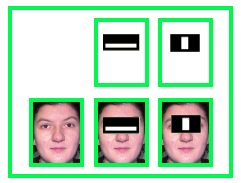
\includegraphics[scale=1]{figures/haar_feature_first_2_features} 
\newline
\caption{The first two Haar features in the original Viola-Jones cascade}
\label{haar_feature_first_2_features}
\end{center} 
\end{figure}

\noindent The structure in itself of the cascade means that within any single image, there is a majority of sub-regions that are negative. This way, since the earliest stage, the cascade tries to reject as many negatives as possible. Because, on the contrary, when a positive instance occurs, it will trigger the evaluation of all the classifiers of the cascade. And this is an really rare event \cite{VIO01}.
\newline

\noindent Following are the different numbers about cascade classifiers (see figure~\ref{haar_feature_cascade_rate}) \cite{UBC01}:

\begin{itemize}
  \item 100\% detection rate and 50\% false positive rate is achieved by a 1 feature classifier
  \item 100\% detection rate and 40\% false positive rate is achieved by a 5 feature classifier
  \item 100\% detection rate and 10\% false positive rate is achieved by a 20 feature classifier
\end{itemize}

\begin{figure}[!h]
\begin{center}
\noindent 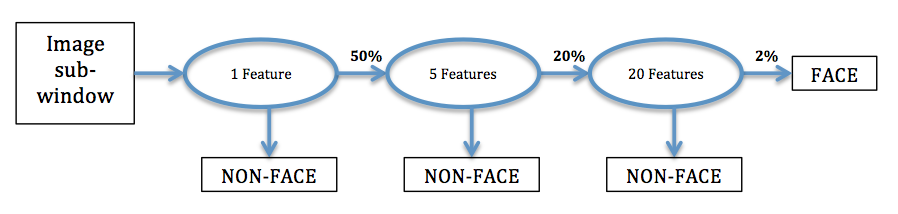
\includegraphics[scale=0.5]{figures/haar_feature_cascade_rate} 
\newline
\caption{Cascade of boosted classifiers rate}
\label{haar_feature_cascade_rate}
\end{center} 
\end{figure}

\phantomsection
\section{Test set and training}

\vspace{\baselineskip}
\noindent The face training set is composed of about 5000 faces (hand labeled). All the faces are scaled and have the same resolution ($ 24\times24 $ pixels). All the faces come from face images on the internet chosen randomly. Some typical face examples are shown in figure~\ref{haar_feature_training_dataset} \cite{VIO01}.
\newline

\begin{figure}[!h]
\begin{center}
\noindent 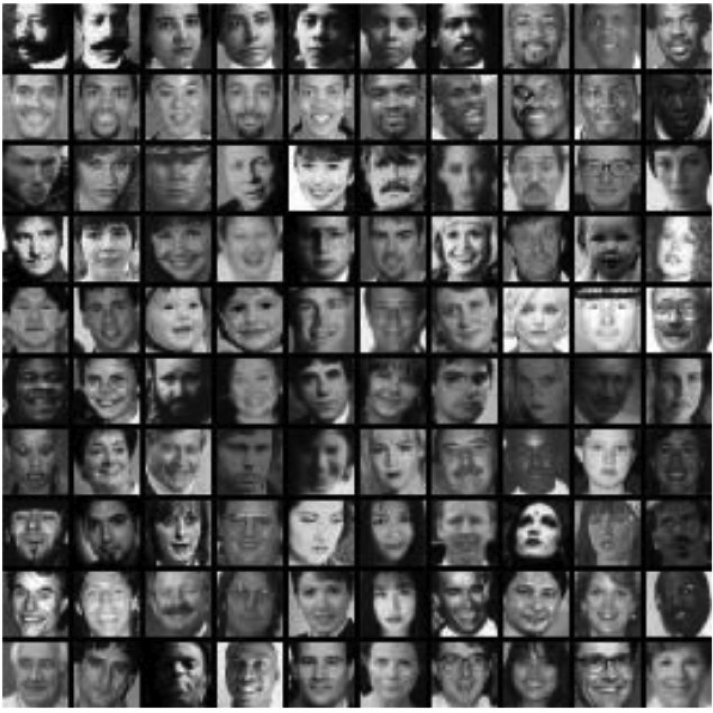
\includegraphics[scale=0.9]{figures/haar_feature_training_dataset} 
\newline
\caption{Example of frontal upright face images used for training}
\label{haar_feature_training_dataset}
\end{center} 
\end{figure}

\noindent To resume, the training set is composed of \cite{UBC01}:

\begin{itemize}
  \item about 5,000 faces
  \begin{itemize}
  	\item All frontal
  \end{itemize}
  \item 300 million non faces sub-regions
  \begin{itemize}
  	\item from 9,400 non-face images
  \end{itemize}
  \item Face are normalized
  \begin{itemize}
  	\item Scale, translation
  \end{itemize}
  \item Many variations
  \begin{itemize}
  	\item Between individuals
	\item Lightning
	\item Pose (rotation of the head)
  \end{itemize}
\end{itemize}

\vspace{\baselineskip}
\noindent Usually, there is two parts into a test set: the first part is the training set and the second part is the validation set. 
Typically, the training set is composed by about 5,000 positives samples (faces) and 10,000 negative samples (non faces: usually it is non face sub-regions chosen from non-face images) \cite{DIN08}. For this kind of training, with a 32 layer classifier the total time is usually of several weeks \cite{VIO01}.
\newline

\noindent Viola-Jones training stage proceeds with the following step \cite{DIN08}:

\begin{itemize}
  \item "Given the number K of possible features (about 160,000 on a $ 24\times24 $ gray-level image)
  \item Fix the number L of desired stages in the cascade
  \item Iterate until L weak classifiers have been selected:
  \begin{itemize}
  	\item Given reweighed data from the previous stage
	\item Train all K weak classifiers (find the best threshold to classify the training set)
	\item Select the best classifier at this stage
	\item Reweight the data"
  \end{itemize}
\end{itemize}

\noindent As said previously, depending on how good a weak classifier is, a weight is associated to it. The weak classifiers are associated to weights that depends on their classification error. The weak classifiers are combined linearly in function of those weights which represents a huge computational cost \cite{DIN08}.
\newline





